
\section{Results}
\label{sec:results}

\noindent
When using mixed-projection treemaps to visualize tree-structured data, the designated use case follows a multi-step process.
First, the user gains overview using the 2D top view on the treemap rendered with orthographic projection.
For all areas-of-interest, the user can select the inner nodes.
Those selected nodes are then tilted into a 2.5D presentation with additional visual variables.
The prototypical implementation is an extension to a 2.5D treemap visualization system by means of
(1) the management of selected inner nodes for the detail view,
(2) computing the nodes' geometry tilting,
(3) efficient image synthesis using an attributed vertex cloud of axis-aligned cuboids where
(4) the tilt is applied during geometry instantiation~\cite{Scheibel2017}.

\subsection*{Application Examples}

\noindent
Mixed-projection treemaps support in getting an overview over a dataset first and finding relevant nodes afterwards by enabling the third dimension on-demand.
As examples of real-world tree-structured datasets we chose a population count dataset and a software system dataset.

\paragraph{Population Count Dataset}
The first dataset is the population count of the zoo in Munich from 2014 (\autoref{fig:example-zoo}).
The dataset contains 247~nodes whereby each node represents one species.
The footprint size of a visual item refers to the population count of a species, the color refers to the extinction threat index, and the number of born animals in the last year is mapped to the height.
This map theme facilitates the detection of recovering species.

\paragraph{Software System Dataset}
The second dataset represents an analysis of the open-source project POCO\footnote{GitHub project available at \url{github.com/pocoproject/poco}; Analysis of revision from March 24 in 2009.} (\autoref{fig:example-poco}).
The dataset contains 5775~nodes.
Each node represents one source code file.
The number of real-lines-of-code is mapped to the footprint size, the color refers to cyclomatic complexity, and the average nesting level of a source code file is mapped to the height.
This map theme is primarily used to detect source code files with disproportional nesting level in comparison to the implemented business logic.

\subsection*{Discussion}
\noindent
While the process is set, the actual depiction of selected nodes is subject to discussion.
There are different approaches for setting the tilt anchor, angle, and additional occlusion-reducing rotation.
To support users in maintaining their mental map, animated transition and different types of perspectives can be applied.

\paragraph{Perspective vs. Orthographic Projection}
Due to perspective foreshortening in a perspective view (the default for virtual 3D environments), objects that are far form the virtual camera away are rendered smaller than closer ones. Alternatively, in an orthographic view, all objects appear at same scale. Since the user preference of projection may differ, both options are supported: (1) perspective projections provide additional information about depth and are often easier to interpret, and (2) orthographic projections facilitate comparison of nodes w.r.t. height and area.
Further, an orthographic projection renders no occlusion to neighboring nodes in the overview.

\paragraph{Tilt Anchor}
After tilting the inner nodes, the inclination introduces unused screen space.
This may be partially covered by higher nodes but the overall impression remains and even supports the identification of these nodes as tilted (and thus, conveying height information).
To exploit this space further, the tilted node can be shifted within the original bounding rectangle (\autoref{fig:tilt-anchor}).
\begin{figure}[h!]
    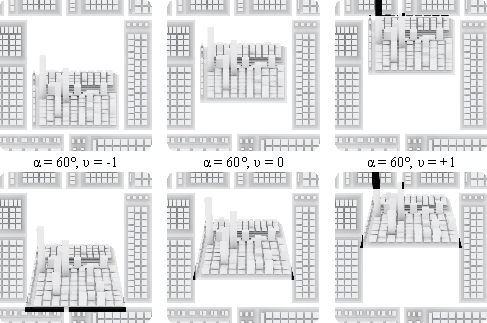
\includegraphics[width=\linewidth]{results-anchor}
    \caption{Orthogonal (top row) and perspective (bottom row) projections anchored at different locations, all tilted by 60° (overdraw colored black).}
    \label{fig:tilt-anchor}
\end{figure}

\noindent
During experiments we made the following observation: the lower alignment seems to be most beneficial as the risk of occluding nearby nodes is minimized (compare to the right pictogram with top alignment; overdraw is colored black) and there is still sufficient space for possible additional information display (as opposed to the center alignment with justified whitespace, compare center pictogram).

\paragraph{Tilt Angle}
The effective tilt angle is subject to inner-node complexity and height-value distribution. Although angles between 0\degree{} and 90\degree{} are possible, a tilt degree of $\alpha= 0\degree$ results in no additional height information and a tilt of $\alpha = 90\degree$yields high occlusion (\autoref{fig:tilt-angle}).
\begin{figure}[h!]
    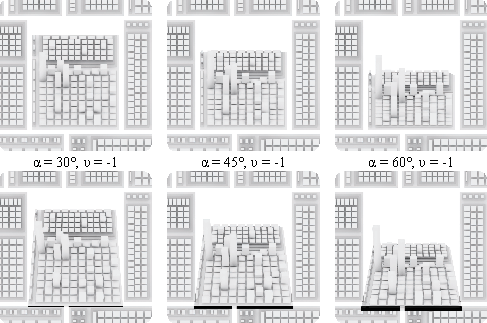
\includegraphics[width=\linewidth]{results-30-45-60}
    \caption{Orthogonal (top row) and perspective (bottom row) projections at different tilt angles, all anchored at the bottom (overdraw colored black).}
    \label{fig:tilt-angle}
\end{figure}
We found tilt angles between $30\degree$ and $60\degree$ to be reasonable supportive.
We also found that a slightly different shading of the cuboids' lateral surfaces servers as additional tilt cue.

\paragraph{Tilt Transitions}
Even though the mixed-projection treemap is designed for static display, the use of manual or animated transitions can help a user to maintain its mental map during the state change from overview to detailed depiction of an inner node and is highly suggested.

\begin{figure}[b!]
    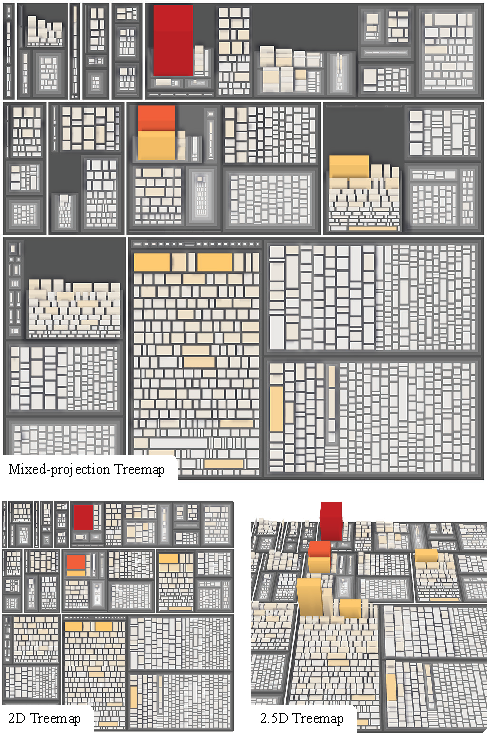
\includegraphics[width=\linewidth]{results-poco}
    \caption{A 2D treemap, 2.5D treemap, and a mixed-projection treemap (with various nodes tilted), all three of which depict the same POCO software system.}
    \label{fig:example-poco}
\end{figure}
